\chapter{路由引擎}\label{routing}

\section{简介}

路由引擎的责任是选择传输的下一跳。一个理想的路由引擎应当可以选择到根节点跳数尽量少而连接质量尽量好的传输路径,这样可以减少转发次数和丢包率,从而降低传感器网络的能量消耗,延长网络的生存期。但由于节点的的存储容量和处理能力一般都非常有限,难以存储大量的路由信息和使用复杂的路由算法,故而有线网络中常用的路由算法如TCP/IP中的OSPF和RIP协议\ucite{stevens1993tii}在这里是不适用的。传感器网络的路由设计注重简单有效,使用有限的资源达到最好的效果。TinyOS 2.x中CTP协议实现的路由引擎可以较好地实现这个目标。它用于建立到根节点的汇聚树,利用链路质量估计器提供的信息合理地选择下一跳节点,使采样节点到根节点的传输次数尽可能地少。

\section{基本概念}
\subsection{路径ETX}
路径ETX(Expected number of Transmissions)是父节点到根节点的ETX与本节点与父节点间的单跳ETX之和,如图\ref{etx-tree}所示。单跳ETX与链路估计器提供的EETX值关系为ETX=EETX+1。它的大小可以反映出到根节点的跳数。在一般情况下,路径ETX越小说明离根节点越近,路由引擎正是根据这一事实选择ETX最小的邻居作为父节点,以期获得到根节点的最少传输次数。
\begin{figure}[ht]
\centering
\begin{tikzpicture}[grow=right, sloped]
\tikzstyle{level 1}=[level distance=3.5cm, sibling distance=3.5cm]
\tikzstyle{level 2}=[level distance=3.5cm, sibling distance=2cm]

\tikzstyle{bag} = [text width=2em, text centered,draw,circle,inner sep=0pt]
\tikzstyle{end} = [circle, minimum width=3pt,fill, inner sep=0pt]
\usetikzlibrary{trees}
\node[bag] {$0$}
    child {
        node[bag] {$4$}        
            child {
                node[end, label=right:
                    {$8$}] {}
                edge from parent
                node[above] {$$}
                node[below]  {$4$}
            }
            child {
                node[end, label=right:
                    {$9$}] {}
                edge from parent
                node[above] {$$}
                node[below]  {$5$}
            }
            edge from parent 
            node[above] {$$}
            node[below]  {$4$}
    }
    child {
        node[bag] {$3$}        
        child {
                node[end, label=right:
                    {$6$}] {}
                edge from parent
                node[above] {$$}
                node[below]  {$3$}
            }
            child {
                node[end, label=right:
                    {$9$}] {}
                edge from parent
                node[above] {$$}
                node[below]  {$6$}
            }
        edge from parent         
            node[above] {$$}
            node[below]  {$3$}
    };
\end{tikzpicture}

\caption{路径ETX值计算}\label{etx-tree}
\end{figure}
\subsection{路由表}
路由表是路由引擎的核心数据结构。CTP协议中使用的路由表结构如图\ref{route-table}所示的形式,它存储了邻居节点信息,主要是邻居的路径ETX值。路由表的大小取决于链路估计器邻居表的大小,因为不在邻居表的节点无法作为邻居节点进入路由表。

\begin{figure}
\centering
\begin{tabular}{|c|c|c|c|}
\hline
\raisebox{-15pt}{邻居节点地址} &\multicolumn{3}{c|}{\raisebox{-8pt}{路由信息}} \\ \cline{2-4}
 &父节点地址 & ETX &  拥塞 \\
\hline
0&&& \\
\hline
1&&& \\
\hline
2&\ldots &\ldots &\ldots  \\
\end{tabular}
\caption{路由表结构}\label{route-table}
\end{figure}


\subsection{CTP路由帧(信标帧)}
路由引擎用广播的形式发送路由帧以便在节点间交换路由信息。

CTP路由帧格式如图\ref{ctp-route-frame}所示:

\begin{figure}[ht]
\centering
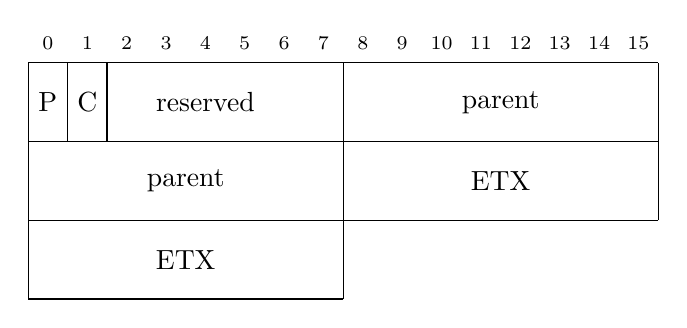
\begin{tikzpicture}
	\pagella
	\draw (0,0) -- (4,0);
	\draw (0,1) -- (8,1);
	\draw (0,2) -- (8,2);
	\draw (0,3) -- (8,3);

	\draw (0,0) -- (0,3);
	\draw (0.5,2) -- (0.5,3);
	\draw (1,2) -- (1,3);
	\draw (4,0) -- (4,3);
	\draw (8,1) -- (8,3);
	\foreach \x in {0,...,15}
	{
	  \draw (\x*0.5+0.25,3.25) node {\scriptsize \x};
	}
	\draw (0.25,2.5) node {P};
	\draw (0.75,2.5) node {C};
	\draw (2.25,2.5) node {reserved};
	\draw (6,2.5) node {parent};
	\draw (2,1.5) node {parent};
	\draw (6,1.5) node {ETX};
	\draw (2,0.5) node {ETX};
\end{tikzpicture}
\caption{CTP路由帧格式}\label{ctp-route-frame}
\end{figure}

各字段意义如下:
\vspace{-10pt}
\begin{itemize}
	\item P:取路由位。如果节点收到一个P位置位的包,它应当尽快传输一个路由帧。
	\item C:拥塞标识。如果节点丢弃了一个CTP数据帧,则必须将下一个传输路由帧的C位置位。
	\item parent:节点的当前父节点
	\item ETX:节点的当前ETX值
\end{itemize}
\vspace{-10pt}
当节点接收到一个路由帧时,它必须更新路由表相应地址的ETX值。如果节点的ETX值变动很大,那么CTP必须传输一个广播帧以通知其它节点更新它们的路由。与CTP数据帧相比,路由帧用父节点地址代替了源节点地址。父节点可能发现子节点的ETX值远低于自己的ETX值的情况,这时它需要准备尽快传输一个路由帧。

\subsection{当前路由信息}
记录当前使用的父节点的信息。如它的AM层地址,路径ETX等。

\section{实现}
TinyOS中路由引擎的实现在\texttt{tos/lib/net/ctp}目录的下列文件中:

\vspace{-10pt}
\begin{itemize}
	\item \texttt{CtpRoutingEngineP.nc}: 路由引擎的具体实现
	\item \texttt{TreeLouting.h}: 路由引擎中使用的一些结构和常数的定义
	\item \texttt{Ctp.h}: 路由帧结构的定义
\end{itemize}
\vspace{-10pt}

\subsection{使用的接口和提供的组件}
从下列源码中可以看到,CtpRoutingEngineP是一个通用组件,可以通过参数设定路由表大小、信标帧发送的最小和最大间隔。它使用了链路估计器、两个定时器和一些包收发处理接口;提供的接口主要是Routing路由接口,它包含了一个最重要的命令nexthop()用于为上层组件提供下一跳的信息。

%\begin{lstlisting}[captionpos=b,caption={\song CtpRoutingEngineP组件使用和提供的接口},label=ctp-routing-engine]
\begin{lstlisting}
generic module CtpRoutingEngineP(uint8_t routingTableSize, 
				uint32_t minInterval, uint32_t maxInterval) {
	provides {
		interface UnicastNameFreeRouting as Routing;
		interface RootControl;
		interface CtpInfo;
		interface StdControl;
		interface CtpRoutingPacket;
		interface Init;
	} 
	uses {
		interface AMSend as BeaconSend;
		interface Receive as BeaconReceive;
		interface LinkEstimator;
		interface AMPacket;
		interface SplitControl as RadioControl;
		interface Timer<TMilli> as BeaconTimer;
		interface Timer<TMilli> as RouteTimer;
		interface Random;
		interface CollectionDebug;
		interface CtpCongestion;

		interface CompareBit;
	}
}
\end{lstlisting}

\subsection{信标帧定时器与路由定时器}
	\subsubsection{信标帧定时器}
	信标帧定时器(BeaconTimer)用于周期性的发送信标帧。发送间隔是指数级增长的。初始的间隔是一个常数minInterval(其值为128),在每更新一次路由信息后,将间隔加倍。因此随着网络的逐渐稳定,将很少看到节点广播信标帧。定时器间隔在使用指数级增长的基础上还加上随机数以错开发送信标帧的时机,避免节点同时发送信标帧导致信道冲突。此外,定时器可以重置为初始值,这主要用于处理一些特殊情况,比如节点收到一个P位置位的包要求尽快发信标帧,或者提供给上层使用者重置间隔的功能。
	\subsubsection{路由定时器}
	路由定时器(RouteTimer)用于周期性的启动更新路由任务。更新间隔固定为一个常数BEACON\_INTERVAL,其值为8192。该定时器触发后将启动更新路由选择任务。

\subsection{发送信标帧与更新路由选择任务}
	\subsubsection{发送信标帧任务}
	由信标帧定时器触发。以广播的方式告知其它节点本节点的ETX值、当前父节点和拥塞信息。
	\subsubsection{更新路由选择任务}
	更新路由选择任务一般由路由定时器触发,但也可以在其它条件下触发,如信标帧定时器到期、重新计算路由、剔除了某个邻居等需要更新路由选择的情况下触发。更新路由选择任务通过遍历路由表找出路径ETX值最小的节点作为父节点,并且该节点不能是拥塞的或是本节点的父节点。

\subsection{信标帧接收事件}
BeaconReceive.receive()事件,在收到其它节点的信标帧时触发。它将根据信标帧的发送者和ETX值更新相应的路由表项。如果收到的是根节点的信标帧,则调用链路估计器将它固定在连接表中。如果信标帧的P位置位,则重设信标帧定时器,以便尽快广播本节点的信标帧让请求者收到。

\subsection{工作流程分析}

路由引擎工作流程如图\ref{route-engine}所示。节点启动时将初始化路由引擎。路由引擎通过将Init接口接到MainC的SoftwareInit接口以实现节点启动时自动初始化路由引擎。初始化的工作有:初始化当前路由信息、初始化路由表为空,初始化路由帧消息缓冲区以及一些状态变量等。

应用程序通过StdControl接口的start()方法正式启动路由引擎,这将启动两个定时器RouteTimer和BeaconTimer。其中RouteTimer的时间间隔设为BEACON\_INTERVAL(8192),BeaconTimer的下一次发送时间初始值设为minInterval(128)。

\begin{figure}[ht]
\centering
\begin{tikzpicture}[>=latex,scale=1.4]
	\draw[->] (0,5.7) -- (0.7,5.7);
	\draw[->] (0,5.7) -- (0,6.3);
	\draw (0,5.8) parabola (0.6,6.2);

	\draw[->] (0,3.7) -- (0.7,3.7);
	\draw[->] (0,3.7) -- (0,4.3);
	\draw (0,3.95) -- (0.6,3.95);

	\draw (1.5,6) circle (0.3);
	\draw (1.5,6) -- (1.8,6);
	\draw (1.5,6) -- (1.5,6.3);

	\draw (1.5,4) circle (0.3);
	\draw (1.5,4) -- (1.8,4);
	\draw (1.5,4) -- (1.5,4.3);

	\draw[->,gray,line width=2pt] (3-0.3,6) -- (3+0.3,6);
	\draw[->,gray,line width=2pt] (3-0.3,4) -- (3+0.3,4);

	\draw (3.5,6.3) rectangle (4.5,5.7);
	\draw (3.8,6.3) -- (3.8,5.7);

	\draw (3.5,3) -- (3.5,4.5) -- (5,4.5) -- (5,3);
	\draw (3.5,3.3) -- (5,3.3);
	\draw (3.5,3.6) -- (5,3.6);
	\draw (3.5,3.9) -- (5,3.9);
	\draw (3.5,4.2) -- (5,4.2);

	\draw (3.9,4.5) -- (3.9,3);
	\draw (4.5,4.5) -- (4.5,3);
	\node at (4.2,4.35) {\tiny ETX};
	\node at (4.2,4.05) {\tiny 9};
	\node at (4.2,3.75) {\tiny 6};
	\node at (4.2,3.45) {\tiny 4};
	\node at (3.7,4.05) {\tiny 2};
	\node at (3.7,3.75) {\tiny 5};
	\node at (3.7,3.45) {\tiny 3};
	\node at (3.7, 3.15) {\tiny\ldots};
	\node at (4.2, 3.15) {\tiny\ldots};
	\node at (4.75, 3.15) {\tiny\ldots};

	\node[draw, circle] (parent) at (5.9,4) {3};
	\node[inner sep=1,circle,fill] (d) at (4.75,3.45) {};
	\draw[->] (d) .. controls +(right:1) and +(left:1) .. (parent);

	\draw[dashed] (7,7) -- (7,2);

	\draw (8,6.3) rectangle (9,5.7);
	\draw (8.3,6.3) -- (8.3,5.7);

	\draw (8,3) -- (8,4.5) -- (9.5,4.5) -- (9.5,3);
	\draw (8,3.3) -- (9.5,3.3);
	\draw (8,3.6) -- (9.5,3.6);
	\draw (8,3.9) -- (9.5,3.9);
	\draw (8,4.2) -- (9.5,4.2);

	\draw (8.4,4.5) -- (8.4,3);
	\draw (9,4.5) -- (9,3);
	\node at (8.7,4.35) {\tiny ETX};
	\node at (8.2,4.05) {\tiny 4};
	\node at (8.2,3.75) {\tiny 1};
	\node at (8.2,3.45) {\tiny 3};
	\node at (8.2, 3.15) {\tiny\ldots};
	\node at (8.7, 3.15) {\tiny\ldots};
	\node at (9.25, 3.15) {\tiny\ldots};

	\node[inner sep=1,fill,circle] (head) at (8.15,6) {};
	\node[inner sep=0] (end) at (8,3.75) {};
	\draw[->] (head) .. controls +(left:1) and +(left:1) .. (end);

	\draw (2.2,6.15) node[text width=1cm,text centered] {\scriptsize 信标帧};
	\draw (2.2,5.85) node[text width=1cm,text centered] {\scriptsize 定时器};
	\draw (2.2,4.15) node[text width=1cm,text centered] {\scriptsize 路由};
	\draw (2.2,3.85) node[text width=1cm,text centered] {\scriptsize 定时器};
	\draw (4.35,4.7) node[text width=1cm,text centered] {\scriptsize 路由表};
	\draw (8.85,4.7) node[text width=1cm,text centered] {\scriptsize 路由表};
	\draw (4,6.5) node[text width=1cm,text centered] {\scriptsize 信标帧};
	\draw (8.5,6.5) node[text width=1cm,text centered] {\scriptsize 信标帧};
	\draw (6,3.15) node[text width=2cm,text centered] {\scriptsize 选择ETX最小};
	\draw (6,2.85) node[text width=2cm,text centered] {\scriptsize 的作为父节点};
	\draw (7.5,3.15) node[text width=1cm,text centered] {\scriptsize 更新路};
	\draw (7.5,2.85) node[text width=1cm,text centered] {\scriptsize 由表项};
	\draw (2,2.4) node {节点1};
	\draw (9,2.4) node {节点2};

	\draw[->,gray,line width=1.5pt] (5,6) -- (7.5,6);
\end{tikzpicture}

\caption{路由引擎工作流程}\label{route-engine}
\end{figure}

由于BeaconTimer的触发时间值设置的比RouteTimer的触发间隔小的多,因此BeaconTimer将率先触发,并投递updateRouteTask()以更新路由选择,接着投递sendBeaconTask()任务发送信标帧。此后,RouteTimer以恒定的时间间隔触发并投递updateRouteTask(),而BeaconTimer触发后会将下次触发的时间间隔加倍。

除了定时器在不断的触发以投递任务外,路由引擎还需要处理其它节点的信标帧。当接收到一个广播的信标帧时,会触发BeaconReceive.receive()事件并根据信标帧中的发送者和它的ETX值更新相应的路由表项。

另外,如果链路估计器剔除了一个侯选邻居,则路由引擎也要相应地从路由表把该邻居移除,并更新路由选择,从而保证了路由表和连接表的一致性。

